%%%% ijcai22-multiauthor.tex

\typeout{IJCAI--22 Multiple authors example}

% These are the instructions for authors for IJCAI-22.

\documentclass{article}
\pdfpagewidth=8.5in
\pdfpageheight=11in
% The file ijcai22.sty is NOT the same as previous years'
\usepackage{ijcai22}

% Use the postscript times font!
\usepackage{times}
\renewcommand*\ttdefault{txtt}
\usepackage{soul}
\usepackage{url}
\usepackage[hidelinks]{hyperref}
\usepackage[utf8]{inputenc}
\usepackage[small]{caption}
\usepackage{graphicx}
\usepackage{amsmath}
\usepackage{booktabs}
\usepackage{algorithm}
\usepackage{algorithmic}
\urlstyle{same}
\usepackage{xcolor}
\usepackage{multicol}
\usepackage{tikz}

\newcommand\todo[1]{\textcolor{red}{#1}}

% the following package is optional:
%\usepackage{latexsym}

\pdfinfo{
	/TemplateVersion (IJCAI.2022.0)
}


\title{A computational approach for variants of coloring planar graphs}

\author{
	Arne Claerhout$^1$\and
	Jorik Jooken$^1$\And
	Jan Goedgebeur$^1$\\
	\affiliations
	$^1$KU Leuven KULAK
	\emails
	arne.claerhout@student.kuleuven.be,
	jorik.jooken@kuleuven.be,
	jan.goedgebeur@kuleuven.be
}


\begin{document}
	
\maketitle

\begin{abstract}
	In this paper, a backtracking algorithm is proposed to color planar graphs according to the proper, odd, conflict-free and unique-maximum vertex colorings.
	
	The chromatic numbers of these coloring variants are also studied further. These are the minimum number of colors needed to color any planar graph.
	Not all chromatic numbers are known, therefore, conjectures exist. This algorithm can be used to disprove or substantiate these conjectures.
	
	The developed algorithm was constructed by applying optimizations to a naive algorithm. The final implementation is a fully optimized algorithm implemented in C.
	
	The proposed algorithm does not outperform alternatives, but is only around $1.4$ times slower for the proper coloring. The algorithm does have the added benefit of easy expandability for other undiscussed coloring variants. No other tools exist for the other coloring variants, therefore, this part of the algorithm can not be compared.
	
	It was found that the conjectures that have not been disproven yet are correct for all planar triangulations with $20$ or less vertices. 
	
\end{abstract}

\section{Introduction}

Graph theory is a field of research in computer science that is older than the computer. Its conception dating back to the 18th century \cite{euler1741solutio}. 

A \textit{graph} $G = (V, E)$ is defined as a pair, containing a collection of vertices ($V$) and edges ($E$). Each edge is an unordered pair of unique vertices. A \textit{planar graph} is a variant of graphs such that a planar embedding is possible without edges crossing. Planar graphs and graphs will be used interchangeably. The \textit{class of planar graphs} $\mathcal{P}$ is defined as the set of all planar graphs. \textit{Planar triangulations}, a subset of planar graphs, are graphs with the maximum number of edges for some number of vertices, this means the addition of an edge would break the planarity of the graph.

The coloring of graphs is one of the most well-known fields in graph theory. A coloring of a graph is a function assigning each vertex a color $1, \dots, k$. The most famous of these colorings is the\textit{ proper coloring}. This states that two vertices sharing an edge, never share the same color. 

The \textit{chromatic number} $\chi(G)$ of a graph $G$ is the minimum number of colors needed to color that graph. A generalization of this is the chromatic number $\chi(\mathcal{P})$ for the class of planar graphs, which is the minimum number of needed colors to color \textit{any} planar graph. For the proper coloring, it was proven that four colors always suffice \cite{appel1976every}. This was a special result, as this was the first ever proof verified using a computer program.

Coloring of graphs has various applications, with uses including: the assignment of frequencies to radio stations, the coloring of maps, scheduling and more.

There exist many variants of graph colorings. One such variant is an \textit{odd coloring}, which was recently introduced by Petruševski and Škrekovski in $2022$ \cite{PETRUSEVSKI2022385}. A proper coloring of a graph is said to be odd if each vertex $v \in V$ has at least one color occurring an odd number of times in its neighborhood $N(v)$. The \textit{odd chromatic number} $\chi_{\mathrm{O}}(\mathcal{P})$ is the minimal number of colors needed to color any planar graph with an odd coloring.

Other variants include conflict-free and unique-maximum colorings. 

The \textit{conflict-free coloring}, introduced in 2003 by Even, Lotker, Ron, and Smorodinsky \cite{even2003conflict}, is a coloring such that every vertex has at least one unique color in its neighborhood, useful because of applications in wireless networks and more \cite{smorodinsky2013conflict}.

To distinguish between different versions of this coloring, neighborhoods of vertices must be defined. An \textit{open neighborhood} of a vertex $v$ is defined as $N(v) = \{w | (v, w) \in E\}$: containing all vertices sharing an edge with $v$, therefore not including the vertex $v$ itself. A \textit{closed neighborhood} of a vertex $v$ is $N[v] = N(v) \cup \{v\}$: the open neighborhood of $v$, including the vertex itself. 

Now consider \textit{proper conflict-free colorings} with respect to open- or closed neighborhoods: a conflict-free coloring where all neighboring vertices have different colors. Depending on which neighborhood definition is used
Both have \textit{chromatic numbers} $\chi_{\mathrm{pCFo}}(\mathcal{P})$ and $\chi_{\mathrm{pCFc}}(\mathcal{P})$ respectively, with the $o$ and $c$ signaling open- or closed neighborhoods.


Similarly, \textit{improper conflict-free colorings} with respect to open- or closed neighborhoods can be defined, the same coloring versions as before, but without the proper constraint. Again, both coloring versions have respective \textit{chromatic numbers} $\chi_{\mathrm{iCFo}}(\mathcal{P})$ and $\chi_{\mathrm{iCFc}}(\mathcal{P})$.

\textit{Unique-maximum colorings} stem from ordered colorings \cite{KATCHALSKI1995141}, and were studied further in the context of open- and closed neighborhoods by Fabrici, Lužar, Rindošová and Soták \cite{fabrici2023proper}. This is a coloring where the maximum color appearing in the neighborhood of a vertex appears exactly once in its neighborhood.

Using the same splitting as the conflict-free coloring, four versions of this coloring can be defined: proper unique-maximum colorings with respect to open- or closed neighborhoods, and improper unique-maximum colorings with respect to open- or closed neighborhoods. Each respectively having their own \textit{chromatic number} for the class of planar graphs: $\chi_{\mathrm{pUMo}}(\mathcal{P})$, $\chi_{\mathrm{pUMc}}(\mathcal{P})$, $\chi_{\mathrm{iUMo}}(\mathcal{P})$ and $\chi_{\mathrm{iUMc}}(\mathcal{P})$.

\subsection{Known bounds}
\label{sec:bounds}

Not all chromatic numbers of these coloring variants are known. For most, only bounds exist, where some upper bound always suffices to color \textit{all} planar graphs, while the lower bound is derived from a graph with the highest \textit{found} chromatic number. 

As the unique color for each vertex $v$ in the $\mathrm{pCFc}$-coloring can always be the color of $v$ itself, this coloring is exactly equal to the proper coloring. Therefore, $\chi_{\mathrm{pCFc}}(\mathcal{P})$ is equal to $4$, the same as the chromatic number of the proper coloring.

The bounds for all coloring variants are as follows:


\begin{itemize}
	\item The odd coloring:
	\begin{itemize}
		\item $5 \leq \chi_{\mathrm{O}}(\mathcal{P}) \leq 8$ (\textit{proven by \cite{petr2023odd} for upper bound, lower bound is $\mathit{C_5}$: cycle of length $5$})
	\end{itemize}
	
	\item The conflict-free colorings:
	\begin{itemize}
		\item $6 \leq \chi_{\mathrm{pCFo}}(\mathcal{P}) \leq 8$ (\textit{proven by \cite{fabrici2023proper}})
		\item $\chi_{\mathrm{pCFc}}(\mathcal{P}) = 4$ (\textit{proven by \cite{appel1976every}})
		\item $4 \le \chi_{\mathrm{iCFo}}(\mathcal{P}) \le 5$ (\textit{proven by \cite{abel2018conflict} for lower bound and \cite{huang2020short} for upper bound})
		\item $\chi_{\mathrm{iCFc}}(\mathcal{P}) = 4$ (\textit{proven by \cite{Malik2023thesis} for lower bound and upper bound is $\mathit{\chi_{\mathrm{pCFc}}(\mathcal{P})}$ because proper coloring is invariably improper})
	\end{itemize}
	
	\item The unique-maximum colorings (all \textit{proven by \cite{fabrici2023proper}}):
	\begin{itemize}
		\item $6 \leq \chi_{\mathrm{pUMo}}(\mathcal{P}) \leq 10$
		\item $6 \leq \chi_{\mathrm{pUMc}}(\mathcal{P}) \leq 8$
		\item $5 \le \chi_{\mathrm{iUMo}}(\mathcal{P}) \le 10$
		\item $4 \le \chi_{\mathrm{iUMc}}(\mathcal{P}) \le 6$
	\end{itemize}
\end{itemize}



\subsection{Conjectures}
\label{sect:Conjectures}

As most of the chromatic numbers are not known. Some authors started formulating conjectures on this problem.

Petruševski and Škrekovski, the originators of the odd coloring, conjectured $\chi_{\mathrm{O}}(\mathcal{P}) = 5$. Other conjectures introduced by Fabrici, Lužar, Rindošová and Soták \cite{fabrici2023proper} include:

\begin{minipage}{0.45\textwidth}
	\raggedcolumns
	\begin{multicols}{2}
		\begin{itemize}
			\item $\chi_{\mathrm{pUMo}}(\mathcal{P}) \leq 7$
			\item $\chi_{\mathrm{pUMc}}(\mathcal{P}) = 6$
			\item $\chi_{\mathrm{iUMo}}(\mathcal{P}) = 5$
			\item $\chi_{\mathrm{iUMc}}(\mathcal{P}) = 4$
			\item $\chi_{\mathrm{pCFo}}(\mathcal{P}) = 6$
			\item $\chi_{\mathrm{iCFo}}(\mathcal{P}) = 4$
			\item $\chi_{\mathrm{iCFc}}(\mathcal{P}) = 3$
		\end{itemize}
	\end{multicols}
\end{minipage}
\vspace{0.4cm}

Since then, the conjecture for the chromatic number of the $\mathrm{iCFc}$-coloring has been disproven, with the exact chromatic number now being known, as shown in Section \ref{sec:bounds}.


\subsection{Research Problem}

In this paper, two research questions are considered:

\begin{itemize}
	\item \textbf{Can we design an algorithm for coloring planar graphs, faster than or just as fast as the existing coloring algorithms, that is also easily expandable to new coloring variants?}
	\item \textbf{In what way is this algorithm useful in helping to prove or disprove conjectures surrounding these coloring variants?}
\end{itemize}

The focus is mostly laid on the design process of the mentioned algorithm. Further results are also discussed.

The structure of this paper is as follows. First, the algorithm developed is discussed in Section \ref{sec:alg} by examining the the pseudocode. Afterwards, the implementation of said algorithm is discussed in Section \ref{sec:implementation}. Here, all notable optimizations applied are studied further. Then, the results of this paper are discussed further in Section \ref{sec:results}. Lastly, the threats to validity are discussed in Section \ref{sec:threats}, ending with the conclusion in Section \ref{sec:conclusion}.


\section{Algorithm}
\label{sec:alg}

In this section, the developed backtracking algorithm is discussed, where the vertices are colored one-by-one and pruning is utilized where possible. The pseudocode is displayed in Algorithms \ref{alg:search}, \ref{alg:check}, \ref{alg:updateN} and \ref{alg:special}. 


We start by explaining Algorithm \ref{alg:search}, the `overseer' of the entire algorithm. It only chooses a maximum color $max\_c$ for the graph and lets the recursive algorithm check if the coloring is possible for that maximum. This is also reflected in the pseudocode. 
Before checking this maximum color, the available colors of the vertices are reset to reflect $max\_c$ (\textit{e.g., if the maximum color is $3$, the available colors will be ${1, 2 \text{ and } 3}$}), as this will be used for early pruning.

Algorithm \ref{alg:check} is the main checking component of the algorithm. It checks whether the given graph $G$ can be colored given a maximum color $max\_c$. This is done in multiple steps, starting with a base case: if all vertices are colored, a valid coloring is reached, which means the chromatic number is found for the graph $G$. 

Otherwise, it loops over all available colors of the given vertex. Here, permutations are avoided, meaning the algorithm makes sure the new color is maximally one higher than the current maximum color in the graph. This optimization is further explained and discussed in Section \ref{sec:optim}.

Next, the $vertex$ is colored with an available color $c$. 
Afterwards, the neighbors of $vertex$ are updated. This is displayed in Algorithm \ref{alg:updateN}, where it updates the neighbors given the newly assigned color $c$ to $vertex$. 

Here, the available colors of all uncolored neighbors of $vertex$ are updated when the coloring $K$ is proper (\textit{e.g., $\mathrm{pUMo}$, odd}), because neighbors can not share the same color for these variants. 

Then, the neighborhoods of the neighbors are checked. If these are fully colored (because the last vertex that was uncolored, $vertex$, was colored this recursion step), the correctness is checked for the coloring $K$. 
The \texttt{update\_neighbors} function is therefore the correctness-checker of the coloring of the graph achieved up until that point. All checks for a valid coloring are done while the graph is being colored, which is why the base case of the algorithm does not check this.

Finally, if the neighborhood of the neighbor still has one vertex left to color, the available colors for this particular vertex are updated. This is achievable for most coloring variants, except the proper coloring. An example is worked out in Algorithm \ref{alg:special} for the odd coloring. Here, the other vertices' colors are used to check compatibility with the available colors of the uncolored vertex $u$. In this case, the odd constraint is checked, if only one color appears an odd amount of times, $u$ can not have this color.
For the other colorings, similar rules are applied to update the vertex $u$.

In case a vertex has no available colors after updating the neighbors, the coloring is not possible anymore and is pruned. The state is reset to before the updates, using \texttt{add\_colors\_back}, and the algorithm backtracks.


If the coloring is still possible after updating the neighbors, the next recursion step is called with a new $index$ and $depth$. 
The new $index$ dictates what vertex to color during the next recursion step. On the other hand, the $depth$ variable is used in the \texttt{add\_colors\_back} function. All changes made in the entire algorithm---meaning \textit{all} updates for \textit{all} vertices during \textit{all} recursion steps---are kept track of. The $depth$ is used to log changes, and easily restore them whenever the coloring is not possible.


% Search
\begin{algorithm}[tb]
	\caption{\texttt{search\_chromatic\_number}}
	\label{alg:search}
	\textbf{Parameters}: The coloring $K$
	
	\textbf{Input}: $\mathcal{G}$: the graphs to color
	
	\textbf{Output}: Chromatic number
	\begin{algorithmic}[1]
		\FOR{\texttt{$G \in \mathcal{G}$}}
		\FOR{$max\_c$ {from} $1$ {to} $\mathbf{MAX}$}
		\STATE \texttt{set\_max\_color\_for\_vertices}($G, max\_c$)
		\IF{\texttt{can\_color\_with\_max\_c}($G, K, 0, max\_c, 0, 0$)} 
		
		\RETURN $max\_c$
		\ENDIF
		\ENDFOR
		\ENDFOR
	\end{algorithmic}
\end{algorithm}

% Check
\begin{algorithm}[tb]
	\caption{\texttt{can\_color\_with\_max\_c}}
	\label{alg:check}
	\textbf{Parameters}: The graph $G$, coloring $K$, max. color in graph $max\_c\_in\_g$, max. color $max\_c$, $index$ and $depth$\\
	\textbf{Output}: Coloring achieved
	\begin{algorithmic}[1]
		\IF{All vertices colored}
		\RETURN true
		\ENDIF
		\STATE $vertex \gets G.vertices$[$index$]
		\FOR{available color $c$ of $vertex$}
		\IF{$\neg$\texttt{is\_UM}($K$) and $c > max\_c\_in\_g + 1$}
		
		\STATE continue
		\ENDIF
		
		\STATE $vertex.color \gets c$
		\STATE $new\_max\_c\_in\_g \gets \max(max\_c\_in\_g, c + 1)$
		
		\IF{\texttt{update\_neighbors}($G, K, vertex, c, depth$)}
		
		\STATE \texttt{add\_colors\_back}($G, depth$)
		\STATE continue
		\ENDIF
		\IF{\texttt{can\_color\_with\_max\_c}($G, K, new\_max\_c\_in\_g,$ $max\_c, $ \texttt{get\_best\_index}()$, depth + 1$)}
		
		\RETURN true
		\ENDIF
		\STATE \texttt{add\_colors\_back}($G, depth$)
		
		\ENDFOR
		
		\STATE $vertex.color \gets 0$
		\RETURN false
	\end{algorithmic}
\end{algorithm}

% update neighbors
\begin{algorithm}[tb]
	\caption{\texttt{update\_neighbors}}
	\label{alg:updateN}
	\textbf{Parameters}: The graph $G$, coloring $K$, $vertex$ to update, color $c$ of $vertex$ and $depth$ of algorithm \\
	\textbf{Output}: Coloring impossible
	\begin{algorithmic}[1]
		\FOR{$n \in $ $vertex.neighbors$}
		
		\IF{\texttt{is\_proper}(coloring $K$) and $n.color = 0$}
		
		\IF{\texttt{remove\_available\_c}($G, n, c, depth$)}
		
		\RETURN true 
		\ENDIF
		\ENDIF
		
		\IF{$n.neighbors$ is fully colored and $\neg$\texttt{is\_correctly\_colored}($K, n$)}
		
		\RETURN true
		\ELSIF{$n.neighbors$ contains only \textbf{one} uncolored vertex $u$}
		\IF{\texttt{handle\_special\_case}($K, u, n.neighbors,$ $ depth$)}
		
		\RETURN true
		
		\ENDIF
		\ENDIF
		\ENDFOR
		\RETURN false
	\end{algorithmic}
\end{algorithm}

% handler
\begin{algorithm}[tb]
	\caption{\texttt{handle\_special\_case\_odd}}
	\label{alg:special}
	\textbf{Parameters}: The coloring $K = $ odd, vertex to update $u$, $neighbors$ and $depth$ \\
	\textbf{Output}: Coloring impossible
	\begin{algorithmic}[1]
		\STATE $colors\_odd = \{\}$
		\FOR{$neighbor \in neighbors \setminus \{u\}$}
		
		\IF{$neighbor.color \in colors\_odd$}
		
		\STATE $colors\_odd = colors\_odd \setminus \{neighbor.color\}$
		
		\ELSE 
		
		\STATE $colors\_odd = colors\_odd \cup \{neighbor.color\}$
		\ENDIF
		
		\ENDFOR
		
		\IF{$\left| colors\_odd \right| = 1$}
		
		\RETURN \texttt{remove\_available\_c}($G, u, colors\_odd, depth$)
		\ENDIF
		\RETURN false
	\end{algorithmic}
\end{algorithm}

It is clear that the algorithm can correctly color graphs, and find the chromatic number of that graph for a given coloring, since all possible colorings are tried and checked, except those that are pruned early.

\section{Implementation}
\label{sec:implementation}

The algorithm was formulated by developing an efficient implementation, and extracting the algorithm from the code. This was done in multiple stages. First, this was developed in Java to test out different data structures and techniques, and to optimize the algorithm. Afterwards, the optimized implementation found in Java, reflecting the algorithm discussed, was ported over to C. All versions of the implementation and other helper scripts are open source\footnote{The \href{https://github.com/ArneClaerhout/color_planar_graphs}{GitHub repository} containing the algorithm.}.

The implementation uses \textit{plantri}, a fast generator of planar graphs developed by Brinkmann and McKay \cite{brinkmann2007fast}. \textit{Plantri} is a tool which can generate all planar graphs for a given number of vertices. This allows the program to easily generate and color graphs simultaneously when some number of vertices is given. 

\subsection{Optimizations}
\label{sec:optim}

Here, the most important optimizations influencing the execution time of the program---all used in the final algorithm discussed previously---are explained. For most optimizations, the impact they have on the runtime is measured to justify the usage. All of the comparisons are measured at the relevant stage of development, such that the code could be kept as clean as possible. A slower ``optimization'' was therefore never implemented again in newer implementations. 

For all experiments, a laptop with an intel i7 CPU was used, using Windows as the OS and WSL to execute the program. Each experiment was performed three times to counteract noise on the data.
All figures used in this section are using these results. Since there are nine \textit{unique} colorings to consider, the cumulative execution time for all coloring variants is used as the performance measure. All times for all colorings are also found here\footnotemark[1].

Results for the different optimizations are found in Figure \ref{fig:general}. Here, the naive algorithm is the simplest algorithm described in Algorithm \ref{alg:naive}, and discussed in Section \ref{sec:correctness}. The other implementations will be discussed further in this section.

\subsubsection{Available colors}

The first optimization used, as already mentioned before, is keeping track of the available colors per vertex. This allows the algorithm to prune early whenever a vertex has no possible colors left. Comparing this to a naive algorithm, yields expected results, shown later. This optimization is only applicable for proper colorings (\textit{e.g., $\mathrm{pUMo}$, proper}). Therefore, the improper coloring variants do not get any speedup. 

\subsubsection{Permutations}

As illustrated in Algorithm \ref{alg:check}, permutations of already tried colorings of the graph are prohibited, except for unique-maximum colorings. For non-unique-maximum colorings, swapping colors (\textit{e.g., changing all vertices with color $2$ to color $3$ and vice versa}) still yields a valid coloring. This dramatically cuts down the search space. 

This isn't the case for a unique-maximum coloring because swapping two colors does not always yield a valid coloring (\textit{e.g., swapping the maximum color with a color occurring twice in a neighborhood}). Therefore, all possible colorings for a graph should be checked for the unique-maximum colorings. 

\subsubsection{Bit-sets}
\label{sec:bitset}

Another optimization used, which is not visible in the pseudocode of the algorithm, is the use of bit-sets. Instead of each vertex having a list of all neighboring vertices as objects, only the indices of the neighbors are stored, which is done in a binary number. If a vertex $v$ has a neighbor with index $i$, the neighborhood bit-set of $v$ has a $1$ at index $i$, starting from the least significant bit. 

This optimization allows for easier comparison between neighborhoods. Checking if some vertex is present in a neighborhood becomes simple, the lookup time is now constant, as this is only a binary operation, instead of a worst-case linear lookup time. 

This optimization, combined with the available colors and permutation optimizations, is implemented in the `optimized' implementation found in Figure \ref{fig:general}. Comparing the naive implementation---a version without these optimizations---to the `optimized' implementation shows the latter performs better, as the time needed stays low for more number of vertices $n$. 

\begin{figure}
	\centering
	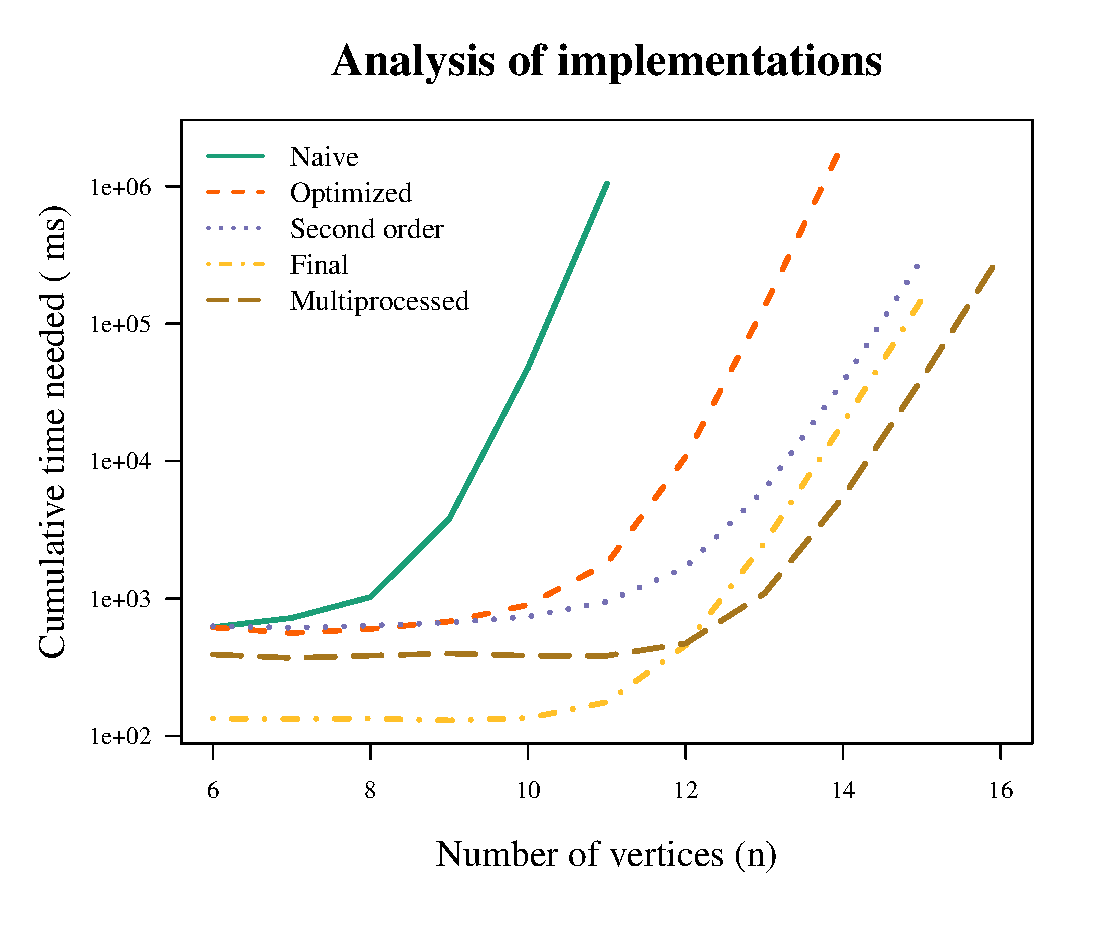
\includegraphics[width=0.45\textwidth]{figures/General_comparison.pdf}
	\caption{A comparison between different versions of the algorithm, tested on all planar triangulations for a given number of vertices. Each implementation performs better than the last.}\label{fig:general}
\end{figure}


\subsubsection{Data structures}

For the implementation of the algorithm, multiple data structures for monitoring vertices were tested.
These include a simple list of vertices, a priority queue and a bit-set implementation. These structures are all discussed because of some strengths each seemingly has. The speed of these data structures are tested against each other.

The list of vertices is a simple data structure, as the updating of a vertex does not demand a change of order in the list. It could therefore work well. The priority queue sorts the vertices by the amount of available colors (from low to high), and therefore has easy lookup for the best vertex to color. And lastly, the bit-set data structure, implemented using a list of bit-sets, where each index of the list denotes a number of available colors. The bit-sets then indicate if a vertex either has or does not have a certain amount of available colors. The last two structures allow the algorithm to find the next optimal vertex to color in constant time, while the list can only do this in worst-case linear time.

The comparison between data structures is found in Figure \ref{fig:datastruct}. It is clear the priority queue method performs the worst. This is because updating the number of available colors requires a completely new entry in the queue, which causes too much overhead. Both the bit-set and standard list implementation perform almost equally well in the figure. But since the scale of the y-axis in the figure is logarithmic, the difference is still substantial. 

This difference is caused by the small overhead the bit-set data structure has in updating the state of a vertex. Whenever the number of available colors changes, the position of that vertex in the data structure should change. The easy lookup for the next vertex to color does not counteract this slow-down enough for bit-sets to perform better than a simple list.

Going forward, the list data structure is used.

\begin{figure}
	\centering
	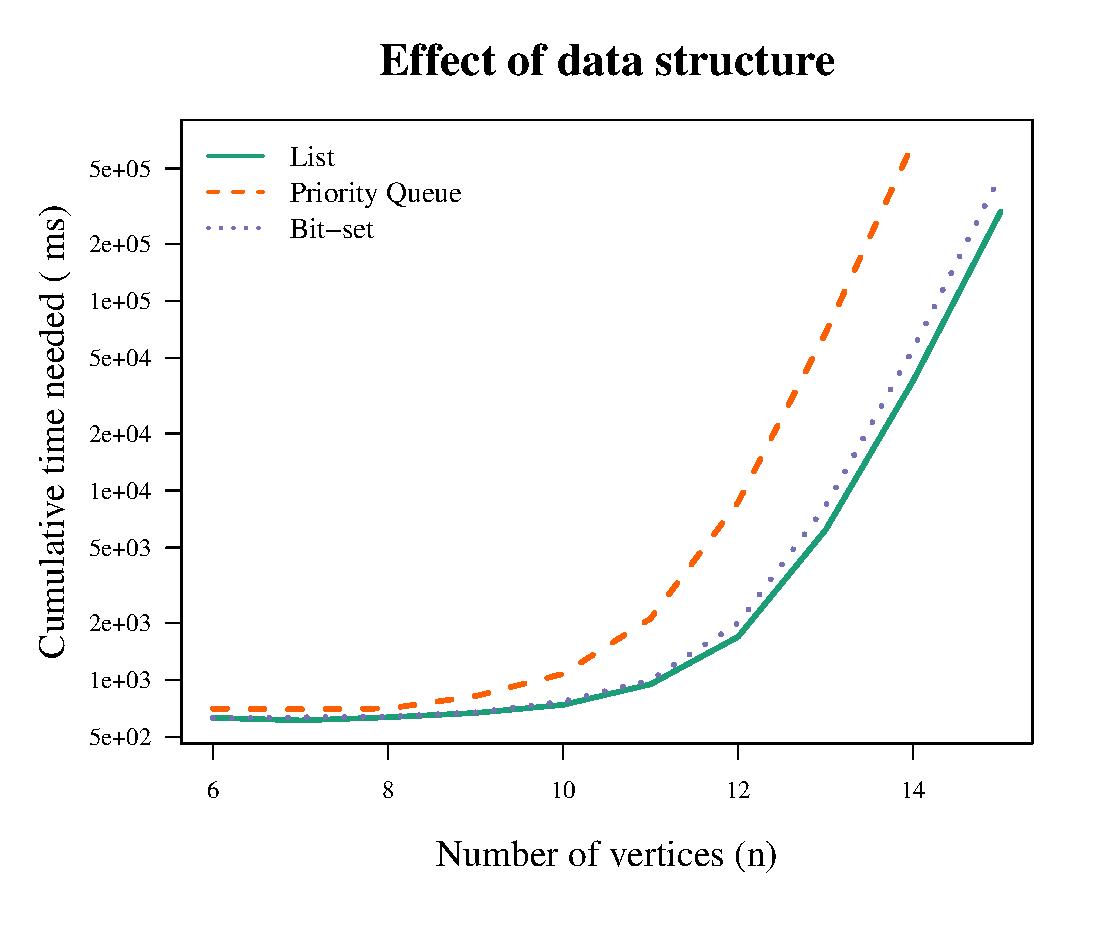
\includegraphics[width=0.45\textwidth]{figures/Datastructures_comparison.pdf}
	\caption{A comparison between the discussed datastructures. The simple list structure performs the best.}\label{fig:datastruct}
\end{figure}

\subsubsection{Index}

In total, five different \texttt{get\_best\_index}-techniques were tested. These techniques range from simply finding the vertex with the least amount of available colors, to finding the vertex with the highest degree. Some methods were adapted from results found by Aslan and Baykan \cite{aslan2016performance}. Only the three best-performing methods are compared here.

Other worse methods mentioned by Aslan and Baykan, such as DSATUR and First Fit either had overhead in registering extra data specifically for the technique, or were too simple and thus already performed badly in the original paper. Therefore, these are not considered in the comparison.

The three best techniques include the two methods mentioned earlier (least number of available colors and highest degree), respectively named Standard and Welsh Powell (WP), and a Standard\_WP-method, a combination of the two: using the Standard technique with a degree tiebreaker. 

Figure \ref{fig:index} shows the comparison of these techniques. Here, there is no doubt that the standard least amount of available colors performs best. It does look like all curves grow as fast for the number of vertices, but the growth phase of the standard technique starts later. Therefore, this index-choosing technique is used from here on out. 

\begin{figure}
	\centering
	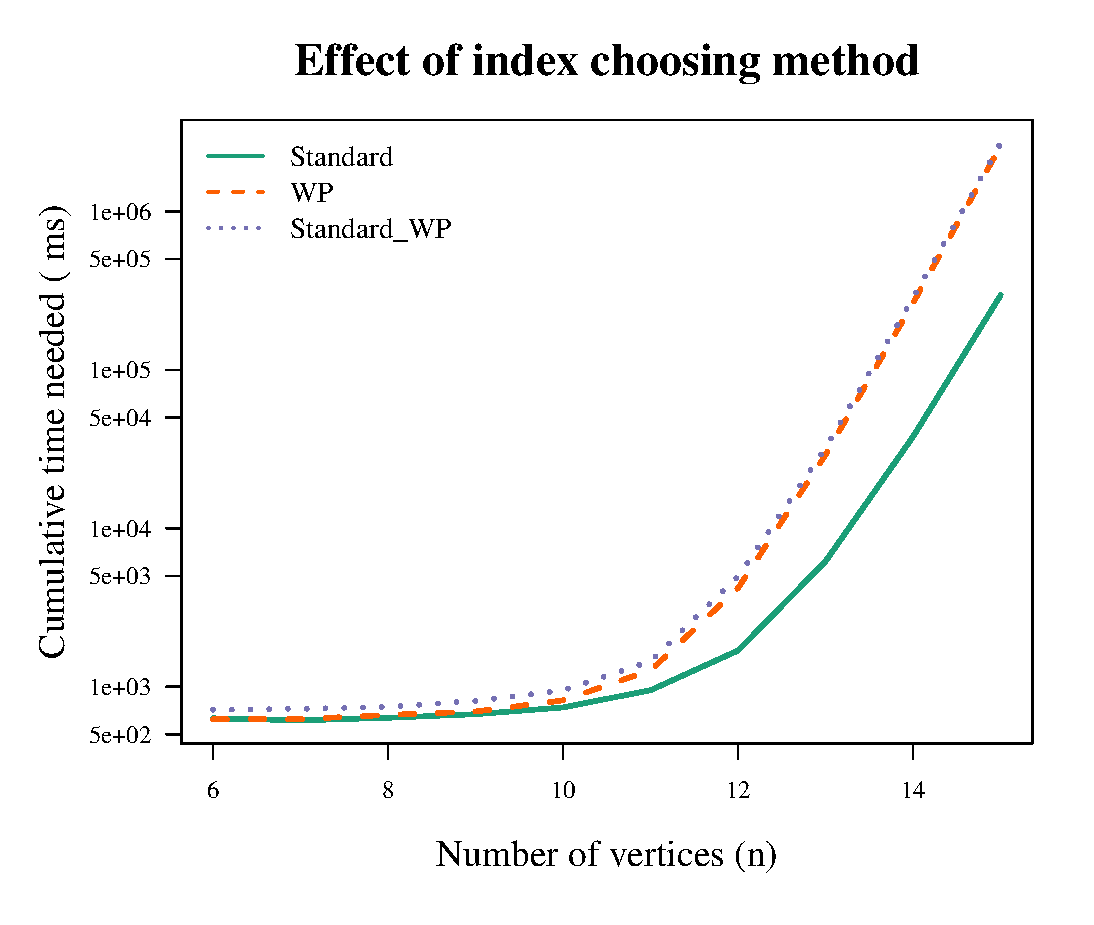
\includegraphics[width=0.45\textwidth]{figures/Index_comparison.pdf}
	\caption{The choosing of next vertex indices is compared for three methods. WP and Standard\_WP perform almost equal. The standard method grows the slowest.}\label{fig:index}
\end{figure}


\subsubsection{Second order optimization}
\label{sec:secondorder}

Instead of only updating the available colors of vertices' neighbors, those of the neighbors' neighbors can also change when coloring a vertex. Here, this is only done when there is only one uncolored vertex left in the neighborhood of the neighbor. One of those rules is displayed in Algorithm \ref{alg:special} for the odd coloring. As mentioned before, the other colorings also have similar rules.

The rule for the unique-maximum coloring checks the number of times the maximum color occurs, if this is only once, prohibit the use of that color, otherwise, the uncolored vertex needs an even higher color to create a new maximum color.

The conflict-free rule checks whether any colors occur once, if not, the uncolored vertex should get a unique color. Otherwise, if there is only one color occurring once, this color should get avoided, if there are multiple, nothing happens. 

The effect of using these second-order optimizations is visible in Figure \ref{fig:general}. This optimization clearly makes the algorithm perform better. It even results in a slower growth of execution time.

\subsubsection{Parallelization}

A simple but effective optimization to apply is the use of parallelization. By using the already provided $RES/MOD$ option in \textit{plantri}---an option to split up the generated graphs into disjoint sets---the coloring of graphs is easily done using multiprocessing: a procedure where a new process is created for each of those independent sets generated. This allows for a significant speedup dependent on the architecture of the system used (\textit{i.e., number of cores}), because now more resources of the CPU can be used.
All outputs are then generated in different output files and combined at finish time.

A comparison between the normal and multiprocessed implementations (run using $10$ processes) is shown in Figure \ref{fig:general}. As expected, for less graphs, splitting up all graphs and combining the results will take longer than simply coloring the graphs. For graphs with more than $12$ vertices, the speedup of using multiprocessing does become apparent. 

\subsubsection{Porting to C}

The last optimization is the moving of the implementation from Java to C. The difference between these two languages lies in the extra overhead found in Java, which uses features like a garbage collector to monitor memory usage. C does not, which allows it to process graphs faster, but it does call for a more careful approach.

Only the best-performing data structures and optimizations are added in C. These are therefore not compared again in C.

Figure \ref{fig:general} shows a comparison between the Java second order implementation and the Final C implementation. The final version does have some extra smaller optimizations, but even comparing both on the exact same implementation will still favor C, as is expected.


\subsection{Correctness}
\label{sec:correctness}

The correctness of the final algorithm is never guaranteed. This is different for very simple versions of the algorithm. By comparing a naive implementation to the final implementation in C, discrepancies in coloring results can get found and resolved. 

% naive
\begin{algorithm}[tb]
	\caption{\texttt{can\_color\_with\_max\_c\_naive}}
	\label{alg:naive}
	\textbf{Parameters}: The graph $G$, coloring $K$, max. color $max\_c$ and $index$ \\
	\textbf{Output}: Coloring achieved
	\begin{algorithmic}[1]
		\IF{$index \ge G.nb\_vertices$}
		
		\RETURN \texttt{is\_correctly\_colored}($G, K$)
		\ENDIF
		
		\FOR{$c$ { from} $1$ {to} $max\_c$}
		
		\STATE $G.vertices$[$index$]$.color \gets c$
		
		\IF{\texttt{can\_color\_with\_max\_c\_naive}($G, K, max\_c, index$)}
		
		\RETURN true
		
		\ENDIF
		
		\ENDFOR
		
		\RETURN false
	\end{algorithmic}
\end{algorithm}

The naive algorithm is displayed in Algorithm \ref{alg:naive}. The code reflects the pseudocode almost one-to-one. Therefore, it is clear that the naive implementation functions by testing every possible coloring given a maximum color. The naive implementation can hence be considered (practically) correct.

Correctness for all planar triangulations with number of vertices $4 \le n \le 12$ were tested for all coloring variants by comparing the final and naive implementations. The improper colorings (\textit{e.g., $\mathrm{iUMc}$}) have lower chromatic numbers overall, therefore these were tested to a maximum of $14$ vertices.
For the proper coloring, an extra tool called \textit{nauty}, developed by McKay and Piperno, is used \cite{mckay2014practical}. This tool can find the chromatic numbers for any graph efficiently. Therefore, more planar triangulations could be tested: those with number of vertices $4 \le n \le 20$.


These tests found correct output, meaning the exact same chromatic numbers, for the final implementation when compared to these more trusted implementations (\textit{nauty} and naive implementation). This gives us high confidence in the correctness of the final implementation.

\section{Results}
\label{sec:results}

Now that the researched problem and the developed algorithm have been discussed, the research questions are revisited. 

The only coloring variant for which any widespread algorithms exist, is the proper coloring. As mentioned before, this includes tools like \textit{nauty}. No open source coloring tool for any of the other colorings exists. This means a comparison for efficiency for all coloring variants is not possible.

Comparing \textit{nauty}'s coloring option against the developed algorithm has expected results. As seen in Table \ref{tab:nauty}, \textit{nauty} is faster in coloring all planar triangulations with some number of vertices. It can be noted that the program developed here is still performing well. Around $1.4$ times slower than \textit{nauty}. For higher number of vertices, the ratio between the two does get smaller, indicating the developed algorithm may be better for graphs with a high number of vertices.


\begin{table}
	\centering
	\begin{tabular}{r|ll|r} 
		\hline
		Number of vertices & This program ($s$) & \textit{Nauty} ($s$) & Ratio \\
		\hline
		$10$ & $0.013$ & $0.003$ & $4.3$ \\ 
		$11$ & $0.014$ & $0.004$ & $3.5$ \\
		$12$ & $0.020$ & $0.008$ & $2.5$ \\
		$13$ & $0.064$ & $0.039$ & $1.64$ \\
		$14$ & $0.39$ & $0.25$ & $1.56$ \\
		$15$ & $2.9$ & $1.9$ & $1.54$ \\
		$16$ & $22$ & $15$ & $1.49$ \\
		$17$ & $177$ & $121$ & $1.46$ \\
		$18$ & $1.4 \times 10^{3}$ & $1.0 \times 10^{3}$ & $1.41$
	\end{tabular}
	\caption{A comparison between the program developed in this paper and \textit{nauty}. Compared for all planar triangulations with a given number of vertices. \textit{Nauty} outperforms this program for all number of vertices. The ratio between the two tools goes down for more number of vertices.}\label{tab:nauty}
\end{table}


\textit{Nauty} is specifically designed for coloring with the proper coloring. The other coloring variants discussed are not supported. These would also require the addition of completely new functions, and a lot of code duplication; or a complete rework of the algorithm. Therefore, \textit{nauty} can not be easily expanded to new colorings, such as those discussed here, whereas this is possible for our developed algorithm. All coloring-dependent methods can be easily expanded without much added work. 

The other colorings are not comparable to other tools. Therefore, profiling the speed or efficiency of the algorithm is hard. But since it compares quite well to \textit{nauty}, and is also very expandable, it does allow us to conclude the algorithm is rather efficient.


The second research question concerned the use of the algorithm for disproving or substantiating conjectures. This is an exhaustive algorithm, therefore, all possible graphs for a given number of graphs can be checked to see if they follow a conjecture or not.

Here, all planar triangulations---graphs with the highest possible number of edges, which therefore have a higher average chromatic number---with $n$ vertices were checked ($4 \le n \le 20$). It was determined that these graphs all conform to the current conjectures on chromatic numbers for all coloring variants. Since planar triangulations are only a subset of all planar graphs, it could still mean there are planar graphs with a higher chromatic number for the same number of vertices $n$ (\textit{e.g., the smallest graph with a chromatic number of $4$ for the $\mathrm{iCFo}$-coloring is not a planar triangulation}). 

Still, only planar triangulations are checked here because the amount of planar graphs grows substantially faster than the number of planar triangulations. There are more planar graphs with only $13$ vertices than planar triangulations with $20$ vertices. 

The program can also assist in disproving the conjectures. An option for the program is provided that will check all possible colorings of a given graph. This allows the user to assert if a graph has a certain property, helping in the search for gadgets: graphs which help in the disproving or proving of some theorem or conjecture. 

The unique-maximum coloring variants have a interesting property useful in the finding of gadgets, which the program can search for. As visible in Figure \ref{fig:graph}, there exist graphs with vertices that always have a certain color. These are great examples of gadgets, findable by the program. This is only applicable to the unique-maximum coloring variants, because as said before, permutations of other coloring variants still lead to a valid coloring. Therefore, for these other variants, no vertex can always have the same color. But, other properties for these colorings are still possible.

\begin{figure}
	\begin{center}
		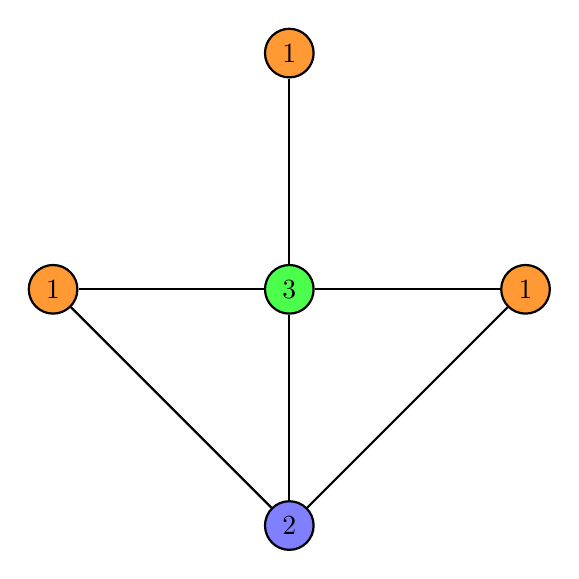
\begin{tikzpicture}[
			% Define the style for the nodes
			every node/.style={circle, draw, thick, minimum size=5mm}
			]
			
			\node (v1) at (0, 0) [fill=blue!50]  {2};
			\node (v2) at (0, 6) [fill=orange!80] {1};
			\node (v3) at (-3, 3) [fill=orange!80]{1};
			\node (v4) at (3, 3) [fill=orange!80]{1};
			\node (v5) at (0, 3) [fill=green!70]{3};
			
			\draw[thick] (v1)--(v3);
			\draw[thick] (v1)--(v4);
			
			\draw[thick] (v5)--(v1);
			\draw[thick] (v5)--(v2);
			\draw[thick] (v5)--(v3);
			\draw[thick] (v5)--(v4);
			
		\end{tikzpicture}
	\end{center}
	\caption{A colored graph for the $\mathrm{pUMo}$ coloring, where each vertex with color $1$ can only have that color. Giving it any other color would result in an invalid coloring.}\label{fig:graph}
\end{figure}


\section{Threats to validity}
\label{sec:threats}

As explained in Section \ref{sec:correctness}, the correctness of the implementation is never guaranteed. Furthermore, the comparison between implementations also does not guarantee correctness for graphs that were never tested, such as graphs with a high number of vertices. 
There is still a possibility that the naive implementation is not implemented correctly. However, this is unlikely because of the perfect reflection between implementation and algorithm. Still, the \texttt{is\_correctly\_colored}-check, seen in Algorithm \ref{alg:naive}, could function incorrectly.

The output of the proper coloring was tested against \textit{nauty}. There is no guarantee of the correctness of \textit{nauty}'s implementation.

All optimization experiments were performed on one specific machine, other computer architectures could yield a different outcome. 
Additionally, comparison of implementation decisions---the optimizations presented---are only tested at one implementation stage (\textit{e.g., naive implementation, post-bit-set implementation}), all tested in Java, and not at each stage of implementation. This could mean that some optimizations applied to the final program may result in different observations. For example, results of optimizations could differ when implemented in C.

\section{Conclusion}
\label{sec:conclusion}

In conclusion, this paper discussed a computational approach for the coloring of graphs. This is done for different variants of vertex colorings: the proper, odd, conflict-free and unique-maximum colorings. 

A backtracking algorithm for coloring planar graphs with these coloring variants is discussed. Firstly, the algorithm was developed in Java, to then be ported over to C for efficiency. In Java, multiple optimizations were tested out and implemented. Different data structures were considered, a simple list performing the best. Additionally, other optimizations such as the usage of bit-sets or parallelization were also considered. 
All optimizations were tested to ensure the optimality of the algorithm.

The correctness of the algorithm was checked by comparing the outputs from the final program to those of a naive version. The simplicity of the naive algorithm combined with identical outputs between the naive algorithm and the final implementation gives us very high confidence in the correctness of the developed program.


This algorithm is the first of its kind, allowing the coloring of graphs for many different variants as one open-source program. It allows users to quickly color in graphs for many different variants, useful in applications such as wireless networks and more.
The program is not as fast as other coloring tools such as \textit{nauty} for the proper coloring. But the easy expandability, something \textit{nauty} lacks, partly makes up for this drawback. 

The conjectures surrounding the chromatic numbers for these colorings were examined further. It was found that the conjectures hold for all planar triangulations with less than or equal to $20$ vertices. This gives some indication that these could hold for more graphs, since planar triangulations---in general---have a higher chromatic number. 


\subsection{Future work}

Future work could include the addition of more coloring variants into the program. This would allow the tool to be used for a wide range of problems. 
Additionally, other versions such as edge-, or face colorings could be included as well.

Next, the algorithm can be more optimized. For example multithreading when coloring one graph with a high number of vertices could speed up the program even further. Furthermore, other coloring rules, such as those described in Section \ref{sec:secondorder}, can be developed.

Lastly, further research could include improving the bounds of the chromatic numbers for the discussed coloring variants. 


\section*{Use of genAI}

For this paper, generative AI was used for the creation of figures. Additionally, it was also used in helping the writing process of the helper bash- and python files used in the implementation (\textit{e.g., color.sh}).

%%%%%%%%%%%%%%%%%%%%%%%%%%%%%%%%%%%%%%%%%%%%


%% The file named.bst is a bibliography style file for BibTeX 0.99c
%\bibliographystyle{named}
\bibliographystyle{plain}
%\bibliographystyle{amsplain}
\bibliography{references}
	
	
\end{document}

